% !TEX encoding = UTF-8 Unicode
\chapter{Minecraft in Education}
\section{Einleitung und Motivation}
In unserer heutigen Gesellschaft wird Medienkompetenz immer wichtiger. Sehr viele Berufe benötigen ein hohes Wissen im Bereich von Fachanwendungen (Office, Adobe etc.) für den Computer. 
Aber auch Menschen mit Berufen, ohne den Einsatz von Computern, werden in Ihrer Freizeit und Umgebung immer mehr von der Digitalisierung betroffen.
Smartphones und Tablets sind mittlerweile allgegenwärtig. An den Hochschulen hat fast jeder Student einen Notebook oder ein Tablet.
Bücher werden durch E-Books ersetzt und Vorlesungs-Unterlagen sind nur noch digital verfügbar. Deshalb ist es umso wichtiger, die nächsten Generationen auf diesen Wandel vorzubereiten. 
Ziel muss es sein, den Umgang mit Medien wie Computern von Klein auf zu üben.

Um dies zu erreichen, soll Wissen spielerisch vermitteln und die bisherigen Medien im Schulsystem durch die neue Generation der Lernspiele erweitert werden.
Bisher waren Lernspiele häufig technisch und spielerisch veraltet (im Vergleich zu modernen Computerspielen) und als Einzelspieler-Spiele konzipiert. Moderne Lernspiele setzten hier auf den Online/Mehrspieler-Aspekt um Gruppenarbeit zu fördern und Schulen miteinander zu vernetzen.

Internationale Unternehmen wie Google, Microsoft und Apple haben erkannt wie wichtig diese neue Form der Lernspiele ist und fördern diese im Schulbereich.
Ein Projekt, auf welches in diesem Kapitel näher eingegangen wird, ist Minecraft in Education.

\section{Projekt Minecraft in Education}

Im Jahr 2009 wurde Minecraft (Version old aplha rd-132211) das erste mal vom
Studio Mojang veröffentlicht. Hauptentwickler war Markus Notch Persson. Zu Beginn wurde Minecraft
ausschließlich über die eigene Webseite des Studios vertrieben und löste bereits nach kurzer Zeit,
einen Hype in der Spielwelt aus. 
\cite{WikiMinecraft}

Minecraft ist ein Computerspiel ohne direktes Spielziel, man spricht von einem \textbf{Sandbox}-Spiel.
Der Spieler übernimmt die Kontrolle über einen Avatar und kann mithilfe von würfelförmigen Blöcken,
in einer 3D-Welt, Konstruktionen erschaffen oder vorhandene bearbeiten. Der Kreativität selbst,
sind dabei kaum Grenzen gesetzt, es gibt eine Vielzahl verschiedener Blockarten mit unterschiedlichen
Eigenschaften. So gibt es Blöcke die physikalisch Korrekt von der Schwerkraft beeinflusst werden,
andere die wiederum in der Luft schweben können und manche die sich wie Flüssigkeiten verhalten.
\cite{WikiMinecraft}

Ein weiterer Grund für die fast unendlichen Möglichkeiten, ist die Erweiterbarkeit des Spiels durch
,von Spielern erstellten, Modifikationen (In der Szene Mods genannt). Mit diesen Erweiterungen ist es
möglich, bis auf das Blocksystem, alle Bereiche des Spieles anzupassen. Einem Weltraumspiel oder einer
Dreidimensionalen Murmelbahn steht nichts im Wege. Neue Arten von Blöcken mit neuen Eigenschaften lassen
sich dabei ebenso einfügen. 

Eine dieser Modifikationen ist das Projekt Minecraft in Education, welches
von Mojang AB und Microsoft Studios gemeinsam entwickelt und Vertrieben wird, mit dem Ziel Minecraft für die Verwendung im Klassenraum anzupassen. \cite{GamepediaMinecraft}

\begin{figure}[ht]
	\centering
	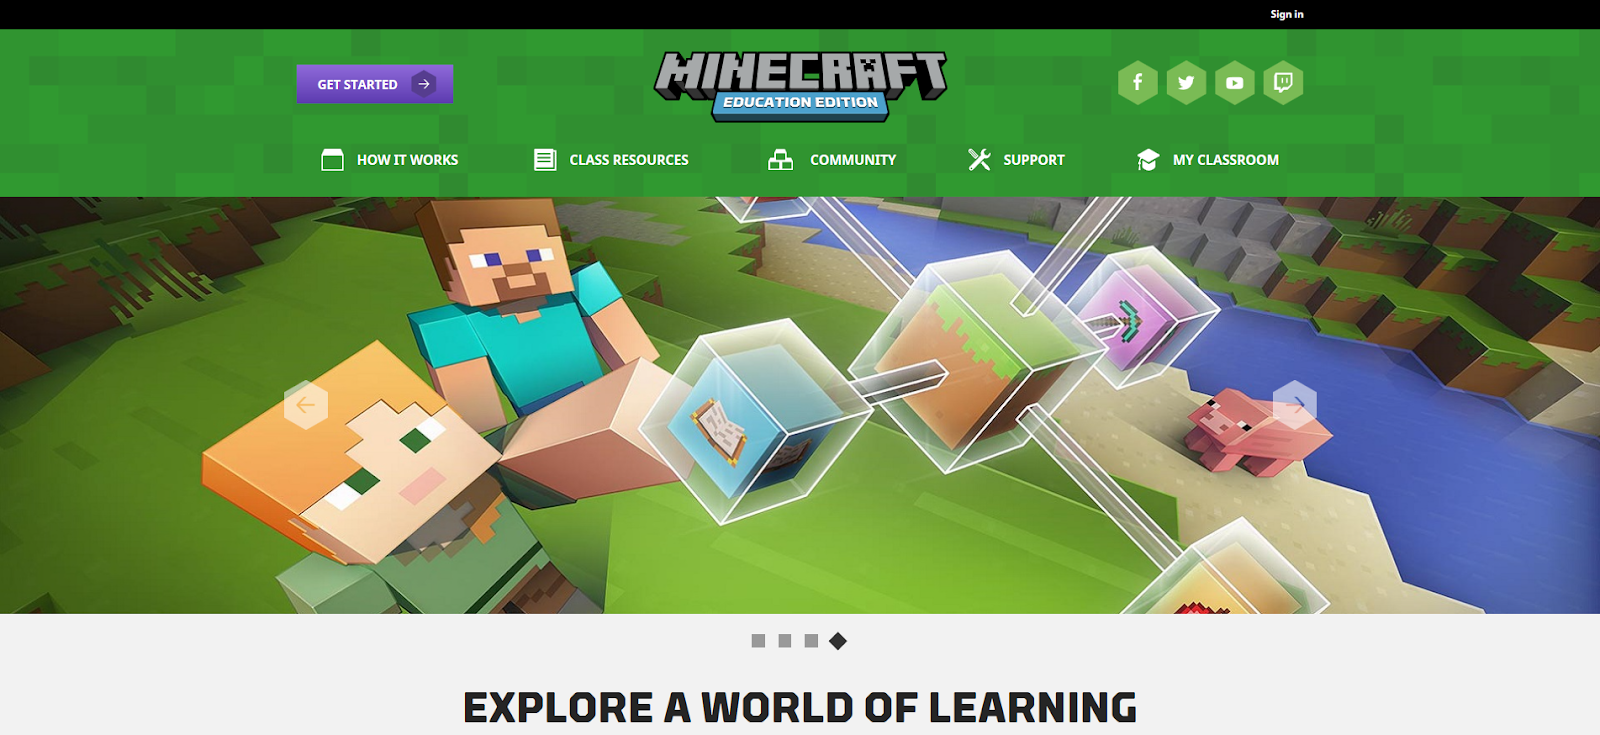
\includegraphics[width=\textwidth,height=\textheight,keepaspectratio]{images/Minecraft.png}
	\caption{Projekt Minecraft in Education}
	\label{projectMinecraft}
\end{figure}

Die erste Version wurde am 1.November 2016 veröffentlicht. Mittlerweile wird es an x Schulen in x Ländern weltweit eingesetzt.
\section{Vernetzung von Schulen}
- Tutoren
- Wissen verteilt
- Unterstützt den Fachkräftemangel abzuschwächen
\section{Virtueller Klassenraum}
- Geschichte Live
- Programmieren lernen
- Physik/Mathematisch praktisch nachvollziehen
- VR Unterstützung für mehr 
\section{Auswirkungen auf das Lernverhalten?}
- Motivation durch Spaß
- Spielerisch Wissen erlangen
- Gruppenarbeit -> Teamfähigkeit!
\section{Gibt es Risiken?}
- Überforderung von Schülern
- Diese Art des Lernens eignet sich nicht für alle Schüler
\section{Erfahrungsberichte}
\section{Fazit}
- Keine neue Lernmethode
- Verbesserte Methode
- Koordination und Lernbereitschaft steigt, durch Spaß am Probieren
- Für viele Fächer geeignet
- Wie alle Medien sollte es unterstützend und nicht als einziges Medium eingesetzt werden